\chapter{Third Party Tools and Resources}

\graphicspath{{../img/ch30/}}


In our solution we have exploited several tools and formalisms. These can be divided into two groups: linguistics and (inductive) logic programming. First we describe the linguistic tools and formalisms, the rest will follow.

\section{Linguistics Analysis} \label{sec:ch30_ling_tools}


\subsection{Prague Dependency Treebank (PDT)}
There exist  
Prague Dependency Treebank related projects   

Homepage of the project: \url{http://ufal.mff.cuni.cz/pdt2.0/}


\begin{figure}
\centerline{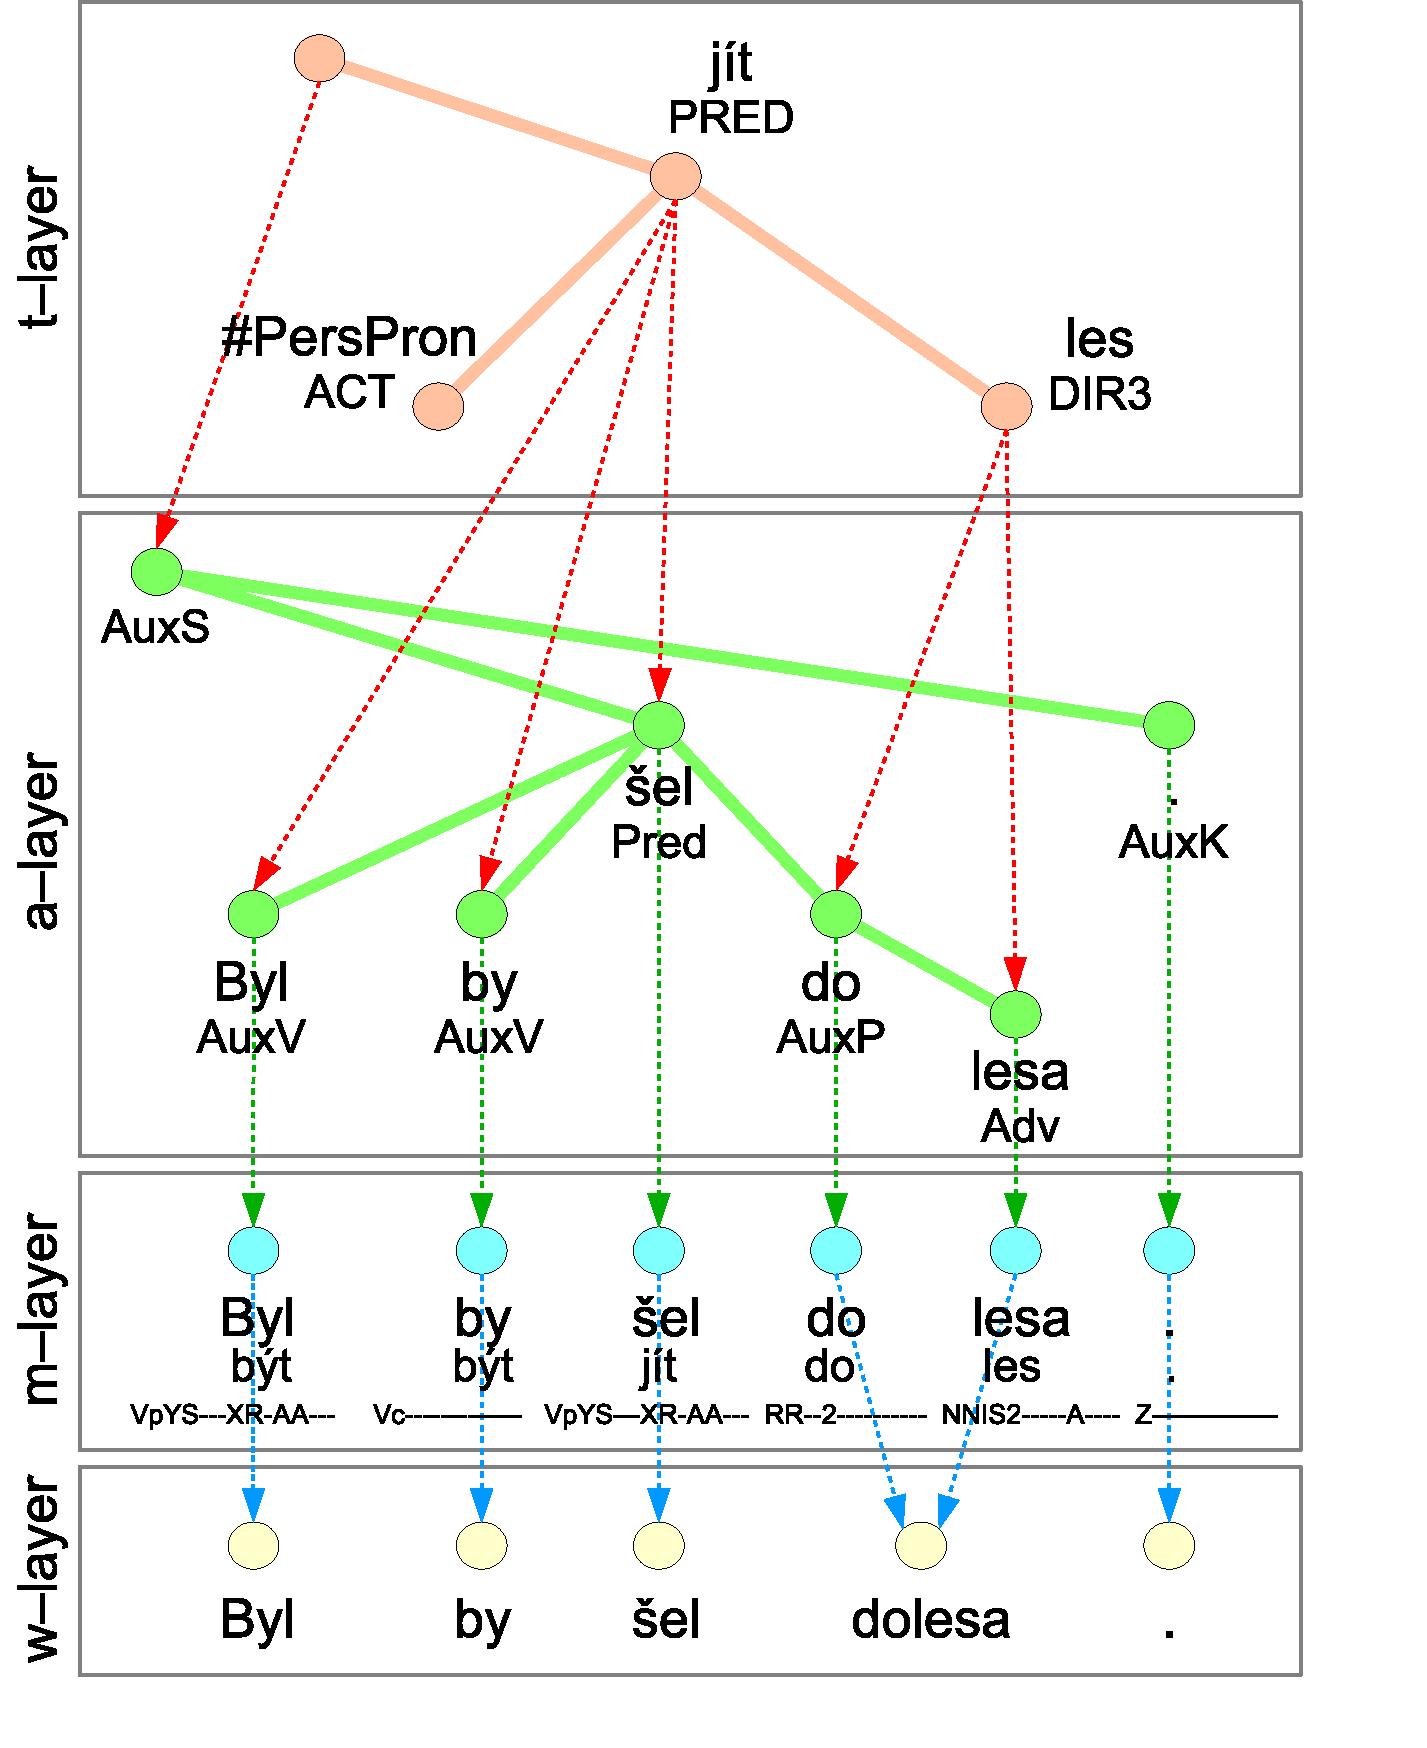
\includegraphics[width=0.6\hsize]{PDT_layers}}
\caption{Layers of linguistic annotation in PDT}
\label{fig:ch30_layers}
\end{figure}


\begin{description}
	\item[Surface layer]
	\item[Morphological layer]
	\item[Analytical layer]
	\item[Tectogrammatical layer]
\end{description}


Sample sentence: Byl by šel dolesa., lit. [He] would have gone intoforest.

Byl by šel dolesa.
\\\[He\] would have gone intoforest.




%%%%%%%%%%%%%%%%%%%%%%%%%%%%%%%%%%%%%%%%%%%%%%%%%%%%%%%%%%%%%%%%%%%%%%%%%%%%%%%%%%%%%%%%%%%%%%%%%
\subsubsection{Linguistic Analysis}
%%%%%%%%%%%%%%%%%%%%%%%%%%%%%%%%%%%%%%%%%%%%%%%%%%%%%%%%%%%%%%%%%%%%%%%%%%%%%%%%%%%%%%%%%%%%%%%%%

In this section we will briefly describe the linguistic tools that we have used to produce linguistic annotations of texts. These tools are being developed in the Institute of Formal and Applied Linguistics\footnote{\url{http://ufal.mff.cuni.cz}} in Prague (ÚFAL), Czech Republic. They are publicly available -- they have been published on a CD-ROM under the title PDT 2.0 \citep{biblio:PDT20_CD} (first five tools) and in \citep{biblio:KlTransformationBasedTectogrammatical2006} (Tectogrammatical analysis). These tools are used as a processing chain and at the end of the chain they produce tectogrammatical \citep{biblio:MiBeAnnotationtectogrammatical2006} dependency trees. Table~\ref{tab:ling_tools} shows some details about these tools. Short descriptions of particular tools follows.


\begin{description}
 
	\item \textbf{Segmentation and tokenization} consists of segmentation (dividing a sequences of tokens into sentences) and tokenization (dividing the input text into words and punctuation).
		
	\item \textbf{Morphological analysis} \citep{biblio:HajicMorfTag} assigns all possible lemmas and morphological tags to particular word forms (word 
occurrences) in the text.
	
	\item \textbf{Morphological tagging} \citep{biblio:HajicMorfTag} consists in selecting a single pair lemma-tag from all possible alternatives assigned 
by the morphological analyzer.
	
	\item \textbf{Collins' parser -- Czech adaptation} \citep{biblio:collinshbrt_1999} Unlike the usual approaches to the description of 
English syntax, the Czech syntactic descriptions are dependency-based, which means that every edge of a syntactic tree captures the relation of dependency between a governor and its dependent node. Collins' parser gives the most probable parse of a given input sentence.
	
	\item \textbf{Analytical function assignment} \citep{biblio:AlyticAsign} assigns a description (\emph{analytical function}, in linguistic sense) to every edge in the syntactic (dependency) tree.
	
	\item \textbf{Tectogrammatical analysis} produces linguistic annotation at the tectogrammatical layer, sometimes called ``layer of deep syntax''. 
	Annotation of a sentence at this layer is closer to the meaning of the sentence than its syntactic annotation; thus, information captured at the tectogrammatical layer is crucial for machine understanding of a natural language \citep{biblio:KlTransformationBasedTectogrammatical2006}.
\end{description}

\begin{table}
\centering
	\begin{tabular}{l|l}
		Name of the tool & Evaluation results (proclaimed by authors) \\[4pt]
		\hline
	Segmentation and tokenization & precision(p): 98,0\%, recall(r): 91,4\% \\[4pt]
	Morphological analysis & 2,5\% unrecognized words\\
	Morphological tagging & 93,0\% of tags assigned correctly \\[4pt]
	Collins' parser -- Czech adaptation & 81,6\% dependencies assigned correctly\\
	Analytical function assignment & precision: 92\% \\[4pt]
	Tectogrammatical analysis & dependencies p:~90,2\%, r:~87,9\%\\
	& assignment of f-tags p:~86,5\%, r:~84,3\%\\
	\end{tabular}
\caption{Linguistic tools for machine annotation}
\label{tab:ling_tools}
\end{table}



\subsubsection{Prague Markup Language (PML)}
\subsubsection{Feature Structure (FS)}


\subsection{Netgraph} \label{sec:ch30_netgraph}

Netgraph \cite{biblio:MiNetgraphA2006} is a linguistic tool used for searching through a syntactically annotated corpus of a natural language (corpus of linguistic dependency trees). Basically Netgraph allows putting restrictions on the shape of a tree and on values of attributes of an arbitrary tree node. Besides that nodes of a query can be marked as optional (not necessarily present in a matching tree) and names can be assigned to query nodes. Naming of query nodes then allows putting restrictions based on referenced nodes (Give me all trees where there is a node with two children and both children have the same lemma.)

See also Section~\ref{sec:ch50_Netgraph_Based_Extraction_Rules}, it provides additional information including example Netgraph queries.

Currently Netgraph is replaced by PML Tree Query (see in the next section) and the Netgraph development is ``discontinued''. We use Netgraph in the present work because it is written in Java, the language of what we use.

Homepage of the project: \url{http://quest.ms.mff.cuni.cz/netgraph/}


\subsection{Tree Editor TrEd, Btred}

TrEd is the ÚFAL key tool for work with dependency based linguistic annotations. It provides a comfortable GUI for navigation, viewing and editing of linguistic trees at different levels if annotation, for different languages and different treebank schemas. 

Homepage of the project: \url{http://ufal.mff.cuni.cz/~pajas/tred/}


\subsubsection{Btred}
TrEd can be also controlled using a powerful set of Perl macros and there is also a non-interactive version of TrEd called Btred, which allows batch evaluation of user macros on an arbitrary set of annotated documents.

\subsubsection{PML Tree Query}
PML Tree Query (PML-TQ) \cite{biblio:PaStSystemfor2009} is a TrEd based module for searching through a treebank using a complex tree based query language.

Homepage of the project: \url{http://ufal.mff.cuni.cz/~pajas/pmltq/}


\subsection{TectoMT}
As we have started with our native language -- Czech (a language with rich morphology and free word order), we had to make tools for processing Czech available in GATE. We have implemented a wrapper for the TectoMT system\footnote{\url{http://ufal.mff.cuni.cz/tectomt/}} \citep{biblio:ZaPtTectoMTHighly2008} to GATE. TectoMT is a Czech project that contains many linguistic analyzers for different languages including Czech and English. We have used a majority of applicable tools from TectoMT: a tokeniser, a sentence splitter, morphological analyzers (including POS tagger), a syntactic parser and the deep syntactic (tectogrammatical) parser. All the tools are based on the dependency based linguistic theory and formalism of the Prague Dependency Treebank project \citep{biblio:PDT20_CD}. So far our solution does not include any coreference and discourse analysis.

Homepage of the project: \url{http://ufal.mff.cuni.cz/tectomt/}

%Czech language
%\\Slavic language, with rich morphology, free word order
%\\Stanford dependencies

\subsection{Czech WordNet}

The Figure~99 shows, that it would be useful to gather words with similar meanings in our extraction rules. For example, the rule in the Figure~99 contains long disjunctions of similar words (nodes with numbers 1 and 4). These disjunctions could be replaced with some kind of expression telling that we are looking for any word from some semantic category (e.g. human beings). For this purpose we wanted to use the Czech WordNet \citep{biblio:WordNetCZ2004}. 

After we have explored the records of the Czech WordNet (CzWN) related to the domain of our interest (car accidents, etc.) we have decided not to involve CzWN in the extraction process. The reason is that the coverage of the vocabulary of our domain is rather poor and the semantic connections of words are sometimes unfortunately missing. But we can supply the missing information to CzWN or we can build up a new domain-specific word-net based on the ground of CzWN.  

Availability: \url{http://catalog.elra.info/product_info.php?products_id=1089}



\subsection{GATE}
GATE\footnote{\url{http://gate.ac.uk/}} \citep{biblio:GATE_ACL2002} is probably the most widely used tool for text processing. In our solution the capabilities of document and annotation management, utility resources for annotation processing, JAPE grammar rules \citep{Cunningham00jape:a}, machine learning facilities and performance evaluation tools are the most helpful features of GATE that we have used.

Homepage of the project: \url{http://gate.ac.uk/}


\section{Weka}

Weka \cite{biblio:Weka} is a well known data-mining software.

Homepage of the project: \url{http://www.cs.waikato.ac.nz/ml/weka/}


\section{Inductive Logic Programming}
Inductive Logic Programming (ILP) \citep{biblio:MuggletonILP} is a machine learning technique based on logic programming. Given an encoding of the known background knowledge (in our case linguistic structure of all sentences) and a set of examples represented as a logical database of facts (in our case tokens annotated with the target annotation type are positive examples and the remaining tokens negative ones), an ILP system will derive a hypothesized logic program (in our case extraction rules) which entails all the positive and none of the negative examples.

See also formal definition of classical ILP task in Section~\ref{sec:ch80_ILP_classic}.

\subsection{ILP tool}
As an ILP tool we have used ``A Learning Engine for Proposing Hypotheses'' (Aleph v5)\footnote{\url{http://www.comlab.ox.ac.uk/activities/machinelearning/Aleph/}}, which we consider very practical. It uses quite effective method of inverse entailment \citep{biblio:InverseEntailment} and keeps all handy features of a Prolog system (we have used YAP Prolog\footnote{\url{http://www.dcc.fc.up.pt/~vsc/Yap/}}) in its background.

Homepage of the project: \url{http://www.comlab.ox.ac.uk/activities/machinelearning/Aleph/}



From our experiments (Section~\ref{sec:evaluation}) can be seen that ILP is capable to find complex and meaningful rules that cover the intended information.



\textbf{?? large amount of training data ??}

As we do not have large amount of training data, there is no problem with excessive time demands during learning and the application of the learned rules is simple and quick.



